\documentclass[conference]{IEEEtran}
\IEEEoverridecommandlockouts
% The preceding line is only needed to identify funding in the first footnote. If that is unneeded, please comment it out.
\usepackage{cite}
\usepackage{amsmath,amssymb,amsfonts}
\usepackage{algorithmic}
\usepackage{graphicx}
\usepackage{textcomp}
\usepackage{xcolor}
\usepackage{comment}
\def\BibTeX{{\rm B\kern-.05em{\sc i\kern-.025em b}\kern-.08em
    T\kern-.1667em\lower.7ex\hbox{E}\kern-.125emX}}

% code listing settings
\usepackage{listings}
\lstset{
    language=Python,
    basicstyle=\ttfamily\small,
    aboveskip={1.0\baselineskip},
    belowskip={1.0\baselineskip},
    columns=fixed,
    extendedchars=true,
    breaklines=true,
    tabsize=4,
    prebreak=\raisebox{0ex}[0ex][0ex]{\ensuremath{\hookleftarrow}},
    frame=lines,
    showtabs=false,
    showspaces=false,
    showstringspaces=false,
    keywordstyle=\color[rgb]{0.627,0.126,0.941},
    commentstyle=\color[rgb]{0.133,0.545,0.133},
    stringstyle=\color[rgb]{01,0,0},
    %numbers=left,
    %numberstyle=\small,
    %stepnumber=1,
    %numbersep=10pt,
    captionpos=t,
    escapeinside={\%*}{*)}
}
%%%----------%%%----------%%%----------%%%----------%%%

\begin{document}

\title{Paper Review-MAP Detection of Misbehaving Relay \\
%{\footnotesize \textsuperscript{*}Note: Sub-titles are not captured in Xplore and
%should not be used}
}

\author{
\IEEEauthorblockN{Harshvardhan Singh}
\IEEEauthorblockA{\textit{Electronics and Comm. Engg.} \\
\textit{Shiv Nadar University}\\
Greater Noida, India \\
hs504@snu.edu.in}
\and
\IEEEauthorblockN{Moesha Malik}
\IEEEauthorblockA{\textit{Electronics and Comm. Engineering} \\
\textit{Shiv Nadar University}\\
Greater Noida, India \\
mm396@snu.edu.in}
\and
\IEEEauthorblockN{Garneni Jhansi}
\IEEEauthorblockA{\textit{Electronics and Comm. Engineering} \\
\textit{Shiv Nadar University}\\
Greater Noida, India \\
}
}

\maketitle

\begin{abstract}
MAP Detection of Misbehaving Relay in Wireless Multiple Access Relay Networks utilises 
or Math in Paper Title or Abstracts.
\end{abstract}

\begin{IEEEkeywords}
Multiple Access Relay Networks, MAP Detection, Misbehaving Relay, bit error, detection
\end{IEEEkeywords}

\section{Introduction}
Network coding is a new relaying technique that replaces the traditional store and forward paradigm of network routing by a method that allows intermediate (relay) nodes to mix the received data before re-transmission. \newline
This has been shown to maximize throughput, as well as robustness. While network coding can be an efficient means of information dissemination in networks, it also presents a new security challenge as a single corrupted packet has the potential to corrupt every packet received by a given destination.\newline
The problem of detecting misbehaving relays that inject false data in single-source networks has been studied in. The receiver then computes the ground truth of the tracing bits and compares them with the tracing bits received from a relay to determine whether it is malicious or cooperative. All these major previous works, however, require sending extra reference data (overhead) at the source to detect the misbehaving relay.  
\section{Previous Works}
The problem of detecting misbehaving relays that inject false data in single-source networks has been studied in the papers referred below:

\subsection{Signatures for Content Distribution}
In \textit{“Signatures for Content Distribution with Network Coding, in Proc. IEEE International Symposium on Information Theory, June 2007"} \cite{b2} the authors consider a peer-to-peer (P2P) network in which the source generates a signature vector and broadcasts to all nodes where it is used to check the integrity of the received packets. The paper proposes a new signature scheme that is based on and is designed specifically for random linear coded systems. The signature scheme makes use of the linearity property of random linear network coding, and enables the peers to check the integrity of packets without the requirement for a secure channel, as in the case of hash function or Secure Random Checksum (SRC) schemes. Also, the computation involved in the signature generation and verification processes is very simple. 

\subsection{Byzantine Modification Detection in Multicast Networks with Random Network Coding}
There are several Information Theory based algorithms proposed for mitigating Byzantine modification attack. In \textit{“Byzantine modification detection in multicast networks with random network coding, IEEE Trans. Inf. Theory, vol. 54, no. 6, pp. 2798-2803, June 2008"} and \textit{"Resilient network coding in the presence of Byzantine adversaries, IEEE Trans. Inf. Theory, vol. 54, no. 6, pp. 2596-2603, June 2008.)"}. Byzantine modification detection capability can be added to a multi-cast scheme based on random linear block network coding, with modest additional computational and communication overhead, by incorporating a simple polynomial hash/check value in each packet.

\subsection{Miscellaneous Methods}
In \textit{“Tracing malicious relays in cooperative wireless communications, IEEE Trans. Inf. Forensics Security, vol. 2, no. 2, pp. 198-212, June 2007"} the authors consider inserting tracing bits in the data stream at the source in a cryptographically secure manner. The receiver then computes the ground truth of the tracing bits and compares them with the tracing bits received from a relay to determine whether it is malicious or cooperative.\newline
Extensions to multiple-source networks have been studied in \textit{“Error analysis in multi-source, multi-relay, multi-destination networks under falsified data injection attacks,” in Proc. IEEE MILCOM, 2008} and \textit{“An algebraic watchdog for wireless network coding, in Proc. IEEE International Symposium on Information Theory, June 2009)}, where the tracing bits or polynomial hash functions are used in detecting the misbehaving relays.

\section{Map Detection Scheme}
The paper proposes the maximum a posteriori (MAP) approach in \textbf{detecting the misbehaving relay that may inject false data}. The MAP detection scheme is \textbf{based on the log-likelihood ratio (LLR) test which is optimal} in the sense of minimizing the probability of incorrect decisions (false alarm and misdetection).
\subsection{Advantages of Scheme}
The given scheme has the following relative advantages to the previously described error detection schemes, which included additional storage (to observe patterns for tampering) and/or transmission overheads (to add parity checks etc.) hence adding to overages which can have significant impact while transmitting large amounts of data. 
\begin{itemize}
\item Does not require sending extra bits at the source, such as hash function or message authentication check bits, and hence there is \textbf{no transmission overhead} 
\item Makes an instantaneous decision about whether a relay is behaving properly without a long term observation. 
\item Derives the probability of \textbf{false alarm and mis-detection as a function of the signal-to-noise ratio (SNR)}, taking into account the lossy nature of wireless links. 
\item Side information regarding the presence of relay misbehavior is exploited at the destination (decoder) to mitigate the relay misbehavior and enhance the reliability of decoding.
\item The MAP decoding scheme exploits the likelihood of the presence of relay misbehavior, and show that it provides a dramatic improvement over the conventional decoder that does not exploit the side information.
\end{itemize}

\subsection{System Model Description}
The system taken under consideration, takes two sources, one relay and one destination (as shown in Fig 1\label{fig1}).We're considering a MA Relay Network, where the source and destination cannot communicate to each other directly because the distance between the source and destination is greater than the transmission range of both of them, hence the need for intermediate node(s) to relay. The relay "overhears" the bits and forwards the coded bit ($p=x_1^r\oplus x_2^r \oplus f$) to the destination. 
\begin{equation}
p = x_1\oplus x_2 \oplus z
\end{equation}
\[where,  z = e_1 \oplus e_2 \oplus f\]
We assume the signals to be sent through orthogonal Rayleigh fading channels with additive white Gaussian noise and path loss
\begin{itemize}
\item Giving us the expression for the received signals at destination as $y_i = h_i*x_i \sqrt{d_i^{-m}* E_s}+n_i , i =1,2$ as received signals from $i^{th}$ source and $y_r = h_r p \sqrt{d_r^{-m} E_r}+n_r$ for the received signal from the relay
\item m is path loss exponent
\item Between the  $i^{th}$ source and destination, and relay and destination:
\begin{itemize}
\item $h_i$ and $h_r$ is channel fading gain (Gaussian variables with mean zero and variance one)
\item $d_i$ and $d_r$ is distance between source and destination, and relay and destination respectively
\item  $E_s$ and  $E_r$ is transmitted energy per symbol
\item  $n_i$ and $n_r$is noise at destination (mean zero and variance $N_o/2$ per dimension)
\end{itemize}
%\begin{figure}
%\centerline{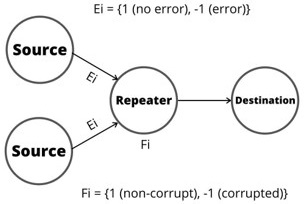
\includegraphics{repeater-diagram.jpg}}
%\caption{Repeater Schematic}
%\label{fig1}
%\end{figure}
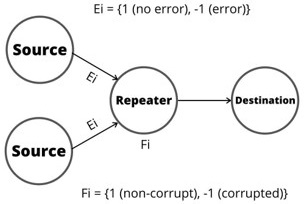
\includegraphics[Fig 1. Repeater Schematic]{repeater-diagram.jpg}


\end{itemize}
\subsection{Detection Rule}
The destination works to find whether $z$ is +1 (well-behaving) or -1 (mis-behaving) to point out if the relay is misbehaving or not. To find out the LLR of $z$ we break it into its constituent component ($p\oplus x_i)$ to find out
\newline LLR of $x_i$ after knowing $h_i$ and $y_i$
\[
\begin{split}
L_i & = ln\frac{P(x_i=+1|h_i,y_i)} {P(x_i=-1|h_i,y_i)} \\
 & = \frac{4\sqrt{d_i^m}}{N_o} Re[h_i^*y_i]
\end{split}
\]
and LLR of $p$, after knowing $h_r$ and $y_r$
\[
\begin{split}
L_r & = ln\frac{P(x_r=+1|h_r,y_r)} {P(x_r=-1|h_r,y_r)} \\
 & = \frac{4\sqrt{d_r^m}}{N_o} Re[h_r^*y_r]
\end{split}
\]
thus deriving our LLR of $z$ as
\begin{equation}
\begin{split}
L(z|h,y)& = ln\frac{P(z=+1|h,y)} {P(z=-1|h,y)} \\
 & \approx sign(L_r*L_1*L_2).min[|L_r||L_1||L_2|] 
\end{split}
\end{equation}
The value of Eqn. 2 will be used to determine the \textbf{estimation} of the value of $z$ as:
\[\hat{z}=+1, \quad if L(z|h,y)\geq 0\]
\[\hat{z}=-1, \quad if L(z|h,y)< 0\]
\begin{lstlisting}[label={list:first},caption=]
def z_estimation_calculate(h,y):
    d_i = 1 # Distance b/w source and relay
    E_s = 1 # Transmit Energy - Source
    d_r = 1 # Distance between relay and reviever
    E_r = 1 # Transmit Energy - Relay
    m = 0.5 # Path loss exponent
    N_o = 0.25 # Variance

    L_r = ((4*pow(d_r,-m)*E_r)/N_o) #To be multiplied by Re[h[0]* y[0]]
    L_1 = ((4*pow(d_i,-m)*E_s)/N_o) #To be multiplied by Re[h[1]* y[1]]
    L_2 = ((4*pow(d_i,-m)*E_s)/N_o) #To be multiplied by Re[h[2]* y[2]]

    sign = lambda a: (a>0) - (a<0)
    sn = sign(L_r*L_1*L_2)
    L_z = sn*min(L_r,L_1,L_2)
\end{lstlisting}

\section{Decoding Schemes}
The paper also places under consideration, three decoding schemes, depending on the side information regarding $z$:
\subsection{MAP Decoder}
The MAP decoder calculates the LLR of $x_1$(or $x_2$) given $h$ and $y$, $L(x_1|h,y)$, and decide $\hat x_1= +1$ if $L(x_1|h,y)>0$ and $\hat x_1= -1$ otherwise. \newline
It considers $(x1, x2, pt \oplus \hat{z})$ as a valid code-word, where $p_t = x1\oplus x2$ is the true parity bit, and finds the most probable (closest) code-word given a received vector (MAP decoding). 
\begin{itemize}
\item Therefore, if a false alarm ($\hat{z}=$ -1 given $z$ = +1) occurs, then the decoder considers (x1, x2, -pt)  as a valid code-word while (x1, x2, pt) is valid. 
\item Similarly, if a miss detection ($\hat{z}$ = 1 given $z$ = -1) occurs, then the decoder considers (x1, x2, pt) as a valid code-word while (x1, x2, -pt) is valid. 
\end{itemize}
In case a wrong parity bit is applied, the reliability of decoding will be decreased.
\begin{lstlisting}[label={list:first},caption=]
def test_z_estimator():
    print("Enter '+1' for binary 1 and '-1' for binary 0")
    x1 = int(input("Enter source 1 output: "))
    x2 = int(input("Enter source 2 output: "))
    p = int(input("Enter relay output: "))
    predict = z_estimation(x1, x2, p)
    if predict >= 0:
        print("Decoded output is +1")
        print(f"Valid code-word: ({x1}, {x2}, +1)")
    elif predict < 0:
        print("Decoded output is -1")
        print(f"Valid code-word: ({x1}, {x2}, -1)")
    else:
        print("Incorrect operation")
\end{lstlisting}
\subsection{Genie Decoder}
The Genie-aided decoder assumes the availability of perfect side information regarding z, i.e. $\hat{z} = z$, hence $P_{FA}=P_{MD}=0$. Therefore, the decoder considers (x1, x2, -pt) as a valid code-word when code-words are generated as (x1, x2,-pt) and, similarly, (x1, x2, pt) as a valid code-word when code-words are generated as (x1, x2, pt). This corresponds to the case of fully cooperative relay (and remains purely theoretical), and serves as a reference for performance comparison with other decoders.
\subsection{Conventional Decoder}
Conventional decoder does not have the side information regarding $z$. Hence, the decoder considers (x1, x2, pt) as a valid code-word no matter what $z$ is. Therefore, if $z$ = -1, the conventional decoder considers (x1, x2, pt) as a valid code-word while (x1, x2,−pt) is valid. Similarly, if $z$ = 1, it considers (x1, x2, pt) as a valid code-word while (x1, x2, pt) is valid. This corresponds to a special case of the proposed decoder with $P_{FA} = 0$ and $P_{MD} = 1$.
\begin{center}
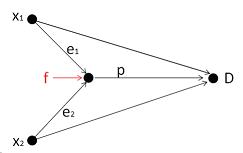
\includegraphics[Fig 2. Decoder Diagram for reference]{fig2.png}
\newline Fig 2. Decoder reference relay diagram
\end{center}
\section{Numerical and Graphical Results}
\subsection{False Alarm and Mis-detection}
The above described system is what is described as a soft-detect system, the paper computes a theoretical probability of false alarm $P_{FA}$ and mis-detection $P_{MD}$ v/s the fraction of energy allotted to each source $\alpha=\gamma_s/\gamma_b$ (where $\gamma_s$ is SNR of each source, and $\gamma_b$ is received SNR per information bit, given by $\gamma_b=(2\gamma_s+\gamma_r)/2 $ 
\begin{lstlisting}[label={list:first},caption=]
def P_Graph():
    for SNR_b in [1,10,100,1000]:
        x=[]
        y=[]
        for i in range(0,100001):
            a=i/100000
            x.append([a])
            SNR_r = 2*(1-a)*SNR_b
            SNR_s = a*SNR_b
            fac = pow(SNR_r/(1+SNR_r),0.5)* (SNR_s/(1+SNR_s))
            P_fa = 0.5*(1-fac)
            y.append([P_fa])
        plt.plot(x,y,label=f"Y_b={int(round(10*math.log(SNR_b,10),0))}dB")
    plt.xlabel('Fraction of Energy per Source, a')
    plt.ylabel('P_FA and P_MD')
    plt.yscale('log')
    plt.legend(loc="lower left")
    plt.grid(True, which="both",ls="dotted")
    plt.show()
\end{lstlisting}

\begin{center}
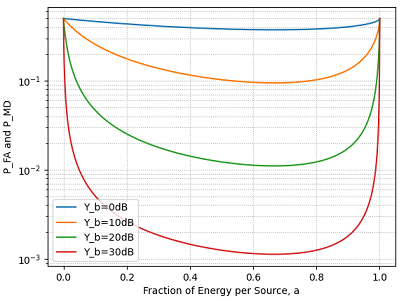
\includegraphics[Graph_1.png]{Graph_1.png}
Fig 3. Probability of false alarm and mis-detection v/s fraction of energy per source
\end{center}



\subsection{Probability of Bit-Error}
Let $\hat x_1$ denote the decoder output for $x_1$ at the destination. The probability of bit error for $x_1$ can be shown to be \cite{b1} (Proof at Appendix A)
\paragraph{MAP Decoder}
\begin{equation}
\begin{split}
P_{E,1} & = P(\hat x_1\neq x_1 | \textbf{h,y})\\
 & = {(1-P_{MD})P(z=-1)+(1-P_{FA})P(z=+1)\over 1+\exp(| L_{1}+L(p\oplus x_{2}| h_{r},y_{r},h_{2},y_{2})|)}\\
 &+ {P_{FA}P(z=+1)+P_{MD}P(z=-1)\over 1+\exp(|L_{1}-L(p\oplus x_{2}| h_{r},y_{r},h_{2},y_{2})|)}
\end{split}
\end{equation}
where 
\[
L(p\oplus x_{2} h_{r}, y_{r}, h_{2}, y_{2}) = \ln{\exp(L_{r})+\exp(L_{2})\over 1+\exp(L_{r}+L_{2})}
\]
and
\begin{equation}
	L(p\oplus x_{2} \oplus (-1)|h_r,y_r,h_2,y_2) = -L(p\oplus x_{2}|h_r,y_r,h_2,y_2)
\end{equation}
 

and a similar method can be used to derived bit error for $x_2$

\begin{itemize}
\item For the case of genie decoder, we can modify Eq. 3 to accommodate for $P_{MD}$=0 and $P_{FA}$=0, to give:]
\begin{equation}
\begin{split}
P_{E,1} & = P(\hat x_1\neq x_1 | \textbf{h,y})\\
 & = {1\over 1+\exp(| L_{1}+L(p\oplus x_{2}| h_{r},y_{r},h_{2},y_{2})|)}\\
\end{split}
\end{equation}
\item And for a conventional decoder, which is a special case of a genie decoder, with $P_{FA}$=0 and $P_{MD}$ =1, and it follows from (3) and (4), that we get
\begin{equation}
\begin{split}
P_{E,1} & = P(\hat x_1\neq x_1 | \textbf{h,y})\\
 & = {P(z=+1)\over 1+\exp(| L_{1}+L(p\oplus x_{2}| h_{r},y_{r},h_{2},y_{2})|)}\\
 &+ {P(z=-1)\over 1+\exp(|L_{1}-L(p\oplus x_{2}| h_{r},y_{r},h_{2},y_{2})|)}
\end{split}
\end{equation}
\end{itemize}
\begin{lstlisting}[label={list:first},caption=]
def BER_estimation_calculate(h, y, SNR_b, a, no):
    L_r = ((4 * pow(pow(d_r, -m) * E_r, 0.5)) / N_o) * (np.conj(h[0]) * y[0]).real
    L_1 = ((4 * pow(pow(d_i, -m) * E_s, 0.5)) / N_o) * (np.conj(h[1]) * y[1]).real
    L_2 = ((4 * pow(pow(d_i, -m) * E_s, 0.5)) / N_o) * (np.conj(h[2]) * y[2]).real

    SNR_r = 2 * SNR_b * (1 - a)
    SNR_s = a * SNR_b

    P_fa = 0.5 * (1 - (pow(SNR_r / (1 + SNR_r), 0.5) * (SNR_s / (1 + SNR_s))))
    P_md = P_fa

    j = math.log((math.exp(L_r) + math.exp(L_2)) / 1 + math.exp(L_r + L_2))  # to find BER for x1
    pf, p1, p2 = 1, 1e-2, 1e-2
    Pz_1 = pf * (1 + 2*p1 + 2*p2 + 3*p1*p2) + (p1 + p2 + 2 * p1*p2)
    Pz1 = 1 - Pz_1
    if no == 1:
        ans = 1 / (1 + math.exp(abs(L_1 + j)))
        return ans
    elif no == 2:
        ans = (((1 - P_md) * Pz_1 + (1 - P_fa) * Pz1) / (1 + math.exp(abs(L_1 + j)))) + ((P_md * Pz_1 + P_fa * Pz1) / (1 + math.exp(abs(L_1 - j))))
        return ans
    elif no == 3:
        ans = (Pz1 / (1 + math.exp(abs(L_1 + j)))) + (Pz_1 / (1 + math.exp(abs(L_1 - j))))
        return ans
\end{lstlisting}

The above BER models can then be plotted for particular values of $\alpha$ (2/3 in this case, for lowest $P_{FA}$ and $P_{MD}$ ) and can be printed using:

\begin{lstlisting}[label={list:first},caption=]
def BER_Graph():  # To print Graph2
    x = []
    y1 = []
    y2 = []
    y3 = []
    a = 2 / 3
    for i in range(0, 161):
        x_no = i/10
        SNR_b = pow(10, x_no)
        x.append([x_no])
        P_E1 = BER_estimation(SNR_b, a, 1)
        y1.append([P_E1])
        P_E1 = BER_estimation(SNR_b, a, 2)
        y2.append([P_E1])
        P_E1 = BER_estimation(SNR_b, a, 3)
        y3.append([P_E1])

    plt.plot(x, y1, label="Conventional")
    plt.plot(x, y2, label="Proposed")
    plt.plot(x, y3, label="Genie-aided")
    plt.xlabel('Received SNR per information bit (in dB)')
    plt.ylabel('Probability of Bit Error (P_E1)')
    plt.yscale('log')
    plt.legend(loc="lower left")
    plt.grid(True, which="both", ls="dotted")
    plt.show()
def BER_estimation(SNR_b, a, no):
    x1, x2, p = -1, -1, -1
    h_r = complex(1, 0.5)
    h_1 = complex(1, 0.5)
    h_2 = complex(1, 0.5)
    y_r = complex(y_calculate(h_r, E_r, p))
    y_1 = complex(y_calculate(h_1, E_s, x1))
    y_2 = complex(y_calculate(h_2, E_s, x2))
    h = [h_r, h_1, h_2]
    y = [y_r, y_1, y_2]
    return BER_estimation_calculate(h, y, SNR_b, a, no)
\end{lstlisting}

\begin{center}
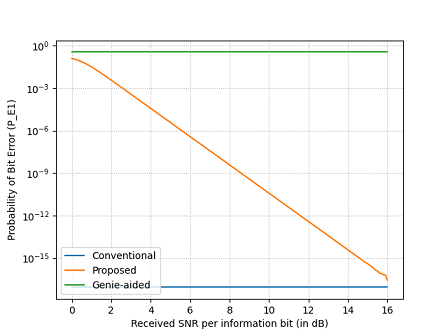
\includegraphics[Graph_2.png]{Graph_2.png}
\newline Fig 4. Probability of Bit-error v/s Recieved SNR per information bit
\end{center}


\section{Scope for further extensions to paper}
Based on the above results, we can extend the scope of the paper to recommend the following extensions to the paper
\paragraph{Reducing number of Sources:} It can be intuitively deduced that with lower number of sources, we face lower chances of the relay admitting a false bit, and consequently lower rate of error
\paragraph{Adding Tracing bits} The process of adding tracing bits involves adding reference bits who's locations are known at the destination. Furthermore, the literature on LLR concludes that for a bit with absolute certainty, the magnitude of LLR for known bit is infinity, thus increasing the total LLR magnitude of {z}.
\paragraph{Adopting better soft-detect methods:} While the LLR detection method has been well-known for being used for soft-detection methods, we can further try and derive additional information about the transmitted data, and based on the kind of data being transmitted factor it in during the decoding stage. 




\begin{thebibliography}{00}
\bibitem{b2} F. Zhao, T. Kalker, M. Medard, and K. J. Han, “Signatures for Content Distribution with Network Coding,” IEEE International Symposium on Information Theory, 2007.
\bibitem{b1} S. W. Kim, “Mitigation of Forwarding Misbehavior in Multiple Access Networks with Network Coding,” IEEE Global Telecommunications Conference GLOBE-COM 2010, 2010.
\bibitem{b0} Yinian Mao and Min Wu, "Tracing Malicious Relays in Cooperative Wireless Communications" 2007 IEEE Transactions on Information Forensics and Security.
 
\end{thebibliography}
\vspace{12pt}
\begin{comment}
\begin{appendices}
\label{appendix:graph}
\section{}
To prove eq. 3, we can adopt a Bayes rule derivation for the same. Let $\hat{x_1}$ denote the decode output $x_1$ at the destination
\[
\begin{split}
P(\hat{x_1}\neq x_1) & =  P(\hat{x_1} \neq x_1 | z=-1)P(z = -1)\\
 &+ {P(\hat{x_1} \neq x_1 | z=+1)P(z = +1) }
\end{split}
\]
From the Bayes rule
\[
\begin{split}
P(\hat{x_1}\neq x_1|z=-1) & =  P(\hat{x_1} \neq x_1 | z=-1)P(z = -1)\\
 &+ {P(\hat{x_1} \neq x_1 | z=+1)P(z = +1) }
\end{split}
\]
\end{appendices}
\end{comment}



\end{document}